\DiaryEntry{Scalar Quantization, 2}{2021-06-16}{Coding}

The basic idea of non-uniform quantization is to quantize signal intervals which have higher probability with more accuracy (closer quantizer intervals) and signals intervals which have lower probability with less accuracy (wider quantizer intervals). On average, the squared error will be reduced.

\subsection{PDF-optimized Quantization}

If we write down the quantization error $\sigma_q^2$,

\be\label{2021-06-16:eq1}
\sigma_q^2 = \int_{- \infty}^\infty (x - Q(x))^2 f_X(x) dx = \sum_i \int_{b_{i-1}}^{b_i} (x - y_i)^2 f_X(x) dx
\ee

then we want to find those values of $b_i, i=0, \ldots M$ and $y_i, i=1, \ldots, M$ that minimize $\sigma_q^2$.

We can actually differentiate above expression wrt to $y_j$ and set it to zero and obtain

\bee
y_j = \frac{ \int_{b_{j-1}}^{b_j} x f_X(x) dx }{ \int_{b_{j-1}}^{b_j} f_X(x) dx }
\eee

The output point for each quantization interval is the centroid of the probability mass in that interval.

In a similar spirit, we can also differentiate wrt to $b_j$, set to zero, and obtain

\bee
b_j = \frac{y_{j+1} + y_j}{2}
\eee

The decision boundary is simply the midpoint of the two neighboring reconstruction levels. Solving these two equations will give us the values for the reconstruction levels and decision boundaries that minimize the mean squared quantization error. Unfortunately, to solve for $y_j$, we need the values of $b_j$ and $b_{j-1}$; and to solve for $b_j$, we need the values of $y_{j+1}$ and $y_j$.

The \emph{Lyod-Max} algorithm solves this problem in an iterative manner.

\subsection{Companded Quantization}

Instead of making the step size small, we could make the interval in which the input lies with high probability large—that is, expand the region in which the input lands with high probability in propor- tion to the probability with which the input lands in this region. This is the idea behind companded quantization.

The following Figure shows a block diagram.

\begin{figure}[H]
    \centering
    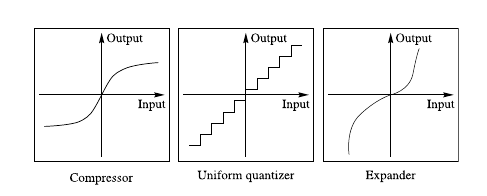
\includegraphics[scale=0.7]{images/2021-06-16-scalar_quant_01.png}
\end{figure}

For the following, we assume that input signal values near zero are more probable than larger input values.

The input is first mapped through a compressor function. This function “stretches” the high-probability regions close to the origin and correspondingly “compresses” the low-probability regions away from the origin. Thus, regions close to the origin in the input to the compressor occupy a greater fraction of the total region covered by the compressor. If the output of the compressor function is quantized using a uniform quantizer and the quantized value transformed via an expander function, the overall effect is the same as using a nonuniform quantizer.

If we bound the source output by some value $x_{max}$, any nonuniform quantizer can always be represented as a companding quantizer. Let us see how we can use this fact to come up with quantizers that are robust to mismatch. First we need to look at some of the properties of high-rate quantizers, or quantizers with a large number of levels. We define

\bee
\Delta_k = b_k - b_{k-1}
\eee

If the number of levels is high, then the size of each quantization interval will be small; and we can assume that the pdf of the input $f_X(x)$ is essentially constant in each quantization interval. Then we have

\bee
f_X(x) = f_X(y_k), \quad \text{if } b_{k-1} \leq x < b_b
\eee

Now we can write the quantization error \eqref{2021-06-16:eq1} as

\bee
\sigma_q^2 = \sum_i \int_{b_{i-1}}^{b_i} (x - y_i)^2 f_X(x) dx \approx \sum_i f_X(y_i) \int_{b_{i-1}}^{b_i} (x - y_i)^2 dx = \frac{1}{12} \sum_i f_X(y_i) \Delta_i^3
\eee

where we used $y_i = \frac{b_i + b_{i+1}}{2}$. 

Let $c(x)$ be a companding characteristic for a symmetric quantizer, and let $c'(x)$ be the derivative of the compressor characteristic with respect to $x$. If the rate of the quantizer is high, (i.e. there are a large number of levels), then within the $k$th interval, the compressor characteristic can be approximated by a straight line segment and the derivative becomes

\be\label{2021-06-16:eq2}
c'(y_k) = \frac{c(b_k) - c(b_{k-1})}{\Delta_k} \rightarrow \Delta_k = \frac{c(b_k) - c(b_{k-1})}{c'(y_k)}
\ee

The expression $c(b_k) - c(b_{k-1})$ is the step size of a uniform $M$-level quantizer. Therefore,

\bee
c(b_k) - c(b_{k-1}) = \frac{2 x_{max}}{M}
\eee

and we can express \eqref{2021-06-16:eq2} as

\bee
\Delta_k = \frac{2x_{max}}{M c'(y_k)}
\eee

We can substitute this expression into \eqref{2021-06-16:eq1} and obtain

\begin{align*}
  \sigma_q^2 &= \frac{1}{12} \sum_i f_X(y_i) \Delta_i^3 = \frac{1}{12} \sum_i f_X(y_i) \left( \frac{2x_{max}}{M c'(y_k)} \right)^3 \\
             &= \frac{x_{max}^3}{3M^2} \sum_i \frac{f_X(y_i)}{c'^2(y_i)} \cdot \frac{2x_{max}}{M c'(y_i)} \\
             &= \frac{x_{max}^3}{3M^2} \sum_i \frac{f_X(y_i)}{c'^2(y_i)} \Delta_i
\end{align*}

For small $\Delta_i$, we can write an integral instead of the sum and obtain the \emph{Bennett integral}

\bee
\sigma_q^2 = \frac{x_{max}^3}{3M^2} \int \frac{f_X(y_i)}{c'^2(y_i)} dx
\eee

The quantizer error depends on the input pdf $f_X(x)$; however, by clever choice of the compander function, we can get rid of this dependency. We chose

\be\label{2021-06-16:eq3}
c'(x) = \frac{x_{max}}{\alpha |x|}
\ee

with some constant $\alpha$. From the Bennett integral we then obtain

\bee
\sigma_q^2 = \frac{x_{max}^3}{3M^2} \int \frac{f_X(y_i)}{c'^2(y_i)} dx = \frac{x_{max}^3}{3M^2} \frac{\alpha^2}{x_{max}^2} \int x^2 f_X(x) dx = \frac{\alpha^2}{3M^2} \sigma_x^2
\eee

with the signal energie $\sigma_x^2 = \int x^2 f_X(x) dx$. We can calculate the SNR as

\bee
SNR = 10 \log \frac{\sigma_x^2}{\sigma_q^2} = \frac{3M^2}{\alpha^2}
\eee

This means that if we use a compressor as defined by \eqref{2021-06-16:eq3}, the SNR of the overall system will be constant regardless of the input signal pdf (and variance). This is quite an interesting and powerful result!

Two companding characteristics that are widely used today are $\mu$-law companding and A-law companding. $\mu$-law is used in North America and Japan, the rest of the world uses A-law characteristic.



%%% Local Variables:
%%% mode: latex
%%% TeX-master: "journal"
%%% End:
